\documentclass[10pt]{article}
\usepackage[a4paper,margin=1in]{geometry}
\usepackage{amsmath,amssymb,amsthm}
\usepackage{booktabs}
\usepackage{hyperref}
\hypersetup{hidelinks}
\usepackage{microtype}
\usepackage{graphicx}
\usepackage{tikz}
\usetikzlibrary{arrows.meta,positioning,fit,calc,shapes.geometric}

\newtheorem{theorem}{Theorem}
\newtheorem{lemma}{Lemma}
\newtheorem{corollary}{Corollary}
\newcommand{\R}{R_q}
\newcommand{\sample}{\mathrel{\leftarrow\joinrel\$}}
\newcommand{\roundp}[1]{\left\lceil #1\right\rfloor_p}

\title{Cut-and-Choose Issuance for Compact Lattice-Based\\
Keyed-Verification Credentials}
\author{Anonymous draft}
\date{Working draft --- security claims are provisional}

\begin{document}
\maketitle

\begin{abstract}
A blind signature lets a user obtain a credential without revealing its
message to the signer.  In the BLNS23 scheme, proving that the user's request
is well formed is expensive because the proof must check hash computations.
We explore replacing this proof with cut-and-choose: prepare several
candidates, reveal some for checking, and use the rest to form the credential.
Our two-message proposal runs this process in parallel \emph{lanes}, each
with its own key, and returns only the sum of their responses.  We describe
how it works, when honest credentials verify, and how many bytes it sends.
We also show how combining earlier responses can produce an extra credential.
With $\kappa$ lanes, the balanced version of this attack costs about
$2^{\kappa/2}$ classical work or $2^{\kappa/4}$ quantum work.  Avoiding this
attack is necessary but does not establish security.  We then give a separate
four-message variant in which the signer chooses what to check after the
user commits.  Its proof keeps one fixed lane valid throughout the issuance
history and reduces the problem of distinguishing aggregate responses from
random to hashed module learning with errors (HMLWE).  Committing every lane
to the same hidden message supports a further argument against producing more
credentials than were issued.  This argument still depends on completing the
protocol simulation and correctness analysis.  Both variants also need a
full privacy proof and concrete secure parameters.
\end{abstract}

\begin{center}
\fbox{\parbox{0.92\linewidth}{\textbf{Security status.}
The two-message proposal has no complete security proof.  The attacks in
Section~\ref{sec:rectangle} show how large its parameters must be to resist
those attacks; larger parameters alone do not prove it secure.  The
four-message variant in Section~\ref{sec:interactive} has a reduction for a
simplified response game.  Extending that result to the full credential
protocol, proving privacy, and choosing secure parameters remain open.}}
\end{center}

\section{Introduction}

A user obtains a credential during \emph{issuance} and later shows it during
\emph{presentation}.  A blind-signature protocol should hide the user's
message during issuance and prevent the signer from linking a later
presentation to that exchange.  In a \emph{keyed-verification} scheme, checking
the credential requires a secret key, usually held by the signer.

BLNS23~\cite{BLNS23} gives such a scheme with small credentials.  Issuance
uses two non-interactive zero-knowledge (NIZK) proofs.  Each proof lets its
recipient check a claim without learning the secret data used to prove it,
and requires no further exchange.  The user's proof $\pi_1$ shows that it
knows short vectors $\mathbf r,\mathbf e_2$ and a message $m$ satisfying
\[
  \rho=H_\rho(\mathbf r,\mathbf e_2),\qquad
  \mathbf c=B\mathbf r+\mathbf e_2+H_R(m,\rho).
\]
Here $\mathbf c$ is the user's blinded request.  The proof checks that it
was formed from a message and small random vectors in the required way.
Without this check, a user could choose a special input, such as a scaled
unit vector, to learn about the signing key.  Checking the hash computations
inside the proof is the main cost we want to remove.

Our proposal uses $\kappa$ \emph{lanes}: parallel copies of this commitment
step, each with its own signing key.  In every lane, the user prepares two
candidate commitments, called \emph{branches}.  A challenge chooses one to
open for checking.  The other is selected for the signer's response.  The
signer evaluates the selected branches and returns only their sum, called the
\emph{aggregate response}.

Each branch is generated from a short random seed.  Revealing that seed lets
the signer reconstruct and check the branch.  A hash of the complete branch
table fixes every branch before the challenge is chosen.  In the two-message
proposal, the user derives the challenge by hashing this commitment, using
the Fiat--Shamir method.  The signer's response proof checks lattice equations
and size bounds, with no hash computation inside the proof.

The credential covers an ordered list of messages
$(m_0,\ldots,m_{\kappa-1})$, one per selected branch.  The message in the
opened branch is a decoy; the selected message stays hidden until
presentation.  An application can hash the ordered list to obtain one
payload.  But because the response adds separate contributions for each
message, earlier responses can sometimes be combined into a new credential.
Section~\ref{sec:rectangle} gives these \emph{splicing attacks}.

We also study a four-message variant.  The signer chooses the challenge
after receiving the user's commitment, and the number of branches per lane
follows a schedule.  This gives the proof a useful guarantee: with high
probability, one fixed lane stays valid throughout all issuances.  Binding
all lanes to the same hidden message then helps rule out extra credentials.
The remaining simulation steps and correctness analysis are still needed to
complete this argument, and privacy needs its own proof.

Section~\ref{sec:security-targets} explains the security goals and the
fixed-lane argument.  Section~\ref{sec:interactive} gives the four-message
variant, and Section~\ref{sec:open} lists the remaining work.  The size
estimates in Section~\ref{sec:efficiency} cover the two-message proposal and
an optional version with more branches per lane.

\section{Notation and basic tools}

We work in the polynomial ring $\R=\mathbb Z_q[X]/(X^d+1)$.  Its elements
have $d$ coefficients, each reduced modulo $q$; multiplication also uses the
rule $X^d=-1$.  Bold symbols denote vectors of $n$ ring elements.  The
notation $\mathbf s^T\mathbf u$ means their inner product: multiply matching
entries and add the results.

The distributions $D_s,D_r,D_e$ sample small secrets and random errors.
We call a vector \emph{short} when it satisfies the required norm bound.
The operation $\roundp{\cdot}$ keeps only the prescribed high-order bits of
each coefficient, giving a result modulo the smaller rounding modulus $p$.
The security parameter is $\lambda$, and the binary proposal has $\kappa$
lanes.  Below, $[\kappa]$ denotes the lane index set
$\{0,\ldots,\kappa-1\}$.

Some proofs use the \emph{random-oracle model} (ROM), which treats a hash as
an ideal random function: a new input gets a random answer, and repeating an
input gives the same answer.  The quantum version (QROM) also allows queries
in superposition.  A classical ROM proof does not automatically cover such
quantum queries.

The balanced splicing attack of Section~\ref{sec:rectangle} costs about
$2^{\kappa/2}$ classically or $2^{\kappa/4}$ with generic quantum search.
Resisting this attack at a 128-bit level therefore requires at least
$\kappa=256$ classically or $\kappa=512$ quantumly.  These are starting
points; a full security bound must also account for other attacks, attempts
against multiple targets, and losses in the reduction.

For lane $i$, the signer samples
\[
  \mathbf s_i\sample D_s,\qquad \mathbf e_{1,i}\sample D_e,
\]
publishes a random matrix $B_i$ and
\[
  \mathbf t_i^T=\mathbf s_i^T B_i+\mathbf e_{1,i}^T.
\]
The keyed verification key is the tuple
$\mathsf{sk}=(\mathbf s_0,\ldots,\mathbf s_{\kappa-1})$.
The verifier needs these separate keys because each lane authenticates a
different hash input.  Keeping only their sum would generally lose the
information needed to verify a credential.

The signer uses one NIZK, $\Pi_{\mathrm{resp}}$, to prove the required lattice
relations for all lanes together.  This proof does not need to show knowledge
of a hash input.  A 384-bit hash $H_{\mathrm{com}}$ binds the branch table:
changing the table while keeping the same digest would require a hash
collision.  Its output length provides approximately 128-bit resistance to
generic quantum collision search.

\section{Two-message construction}\label{sec:construction}

\subsection{Preparing and committing to the branches}

The user independently constructs two branches $b\in\{0,1\}$ in each lane
$i\in\{0,\ldots,\kappa-1\}$.  It samples a 32-byte seed $z_{i,b}$ and expands it with an extendable-output
function (XOF), which produces as many pseudorandom bytes as needed.  Separate
labels distinguish the uses of this function.  A fixed sampling procedure
turns those bytes into
\[
 (m_{i,b},\mathbf r_{i,b},\mathbf e_{2,i,b})
 =G(\mathsf{sid},i,b,z_{i,b}),
\]
where $m_{i,b}$ is 32 bytes and the two vectors have the prescribed bounded
distributions.  It computes
\begin{align*}
 \rho_{i,b}&=H_\rho(\mathsf{sid},i,b,
                     \mathbf r_{i,b},\mathbf e_{2,i,b}),\\
 \mathbf u_{i,b}&=H_R(\mathsf{credential\mbox{-}lane},i,m_{i,b},\rho_{i,b}),\\
 \mathbf c_{i,b}&=B_i\mathbf r_{i,b}+\mathbf e_{2,i,b}
                   +\mathbf u_{i,b}.
\end{align*}
The session identifier $\mathsf{sid}$ identifies the protocol version, issuer,
and key epoch (the period using the same set of keys).  It also includes fresh
values from both parties.  The user hashes the complete branch table in a
fixed order:
\[
 C=H_{\mathrm{com}}(\mathsf{protocol},\mathsf{issuer},\mathsf{pk},
       \mathsf{sid},
       \mathsf{Encode}(\mathbf c_{0,0},\mathbf c_{0,1},\ldots,
                       \mathbf c_{\kappa-1,0},\mathbf c_{\kappa-1,1})).
\]
The encoding records the branch count, dimensions, and lengths so that it has
only one interpretation.  This single 48-byte digest commits the user to all
$2\kappa$ branches and their order before the challenge is chosen.

\subsection{Choosing and checking the open branches}

After all commitments are fixed, the user derives
\[
 \boldsymbol\chi=(\chi_0,\ldots,\chi_{\kappa-1})
 =H_{\mathrm{chal}}(\mathsf{protocol},\mathsf{issuer},\mathsf{pk},
   \mathsf{sid},C)
 \in\{0,1\}^{\kappa}.
\]
In lane $i$, the user reveals seed $z_{i,\chi_i}$ so that the signer can
check branch $\chi_i$.  For the other branch, the user sends the full vector
$\mathbf c_{i,1-\chi_i}$ and keeps its seed private.

The signer recomputes the challenge from $C$ and checks that the seeds and
vectors have the assigned roles.  It expands every revealed seed and combines
the reconstructed branches with the received vectors in the agreed order.
It then hashes all $2\kappa$ branches and checks that the result equals $C$.
For each opened branch, it also checks the hash computations, lattice
equation, size bounds, encoding, and function labels.  If any check fails,
it stops without returning a value that depends on its secret key.  We call
$b_i^*=1-\chi_i$ the \emph{selected branch} and write
$\mathbf c_i^*=\mathbf c_{i,b_i^*}$ for its vector.

The selected seeds stay private even at presentation.  The user reveals only
$(m_i^*,\rho_i^*)$: a selected seed would also reveal the blinding vectors
$\mathbf r_i^*,\mathbf e_{2,i}^*$ and let the issuer match the credential to
its issuance exactly.  Implementations must agree on the XOF, sampling
order, byte encoding, and iteration limits so that the same seed always
recreates the same branch.

Thus issuance has the two-message form
\[
 \mathsf{User}\longrightarrow\mathsf{Signer}:
 C,
 \{z_{i,\chi_i},\mathbf c_{i,1-\chi_i}\}_i,
 \qquad
 \mathsf{Signer}\longrightarrow\mathsf{User}:h,\pi_{\mathrm{resp}}.
\]
Fiat--Shamir saves an exchange with the signer, but the user can try many
branch tables locally until the hash gives a favorable challenge.  This
search is called \emph{grinding}.  Fixing $k$ chosen challenge bits takes
about $2^k$ classical random-oracle queries or $2^{k/2}$ generic quantum
queries.  The quantum security analysis must account for this search.  A
fresh random value from the signer limits work done in advance, but costs
another message unless an authenticated session setup already provides it.

\begin{figure}[t]
\centering
\resizebox{\linewidth}{!}{%
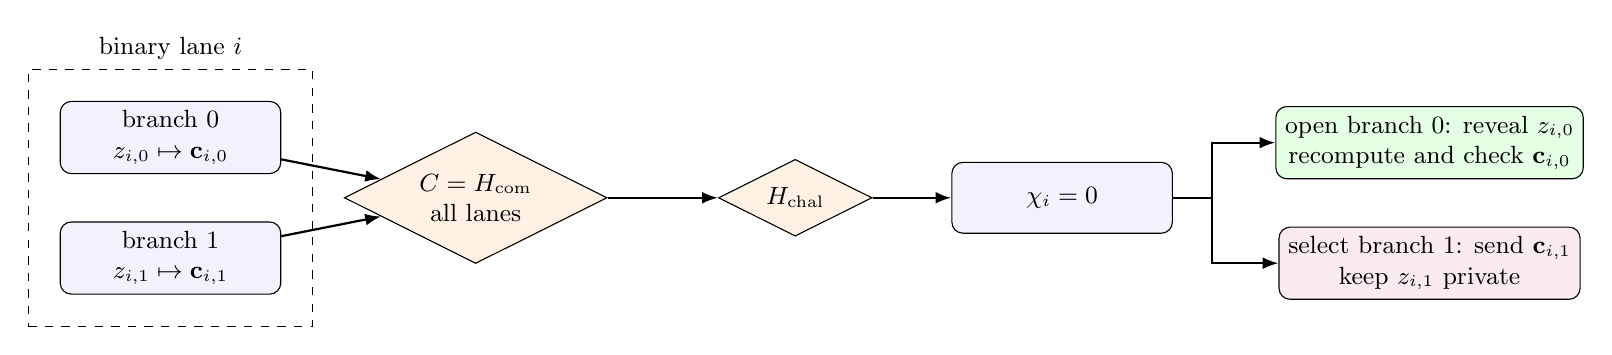
\begin{tikzpicture}[
  font=\small,
  node distance=6mm and 10mm,
  box/.style={draw,rounded corners,align=center,minimum height=9mm,
              minimum width=28mm,fill=blue!5},
  hash/.style={draw,diamond,aspect=2,align=center,fill=orange!10},
  ok/.style={draw,rounded corners,align=center,fill=green!10},
  keep/.style={draw,rounded corners,align=center,fill=purple!8},
  arrow/.style={-{Latex[length=2mm]},thick}
]
\node[box] (b0) {branch $0$\\$z_{i,0}\mapsto\mathbf c_{i,0}$};
\node[box,below=of b0] (b1) {branch $1$\\$z_{i,1}\mapsto\mathbf c_{i,1}$};
\node[hash,right=22mm of $(b0)!0.5!(b1)$] (com) {$C=H_{\rm com}$\\all lanes};
\node[hash,right=14mm of com] (chal) {$H_{\rm chal}$};
\node[box,right=of chal] (chi) {$\chi_i=0$};
\draw[arrow] (b0) -- (com);
\draw[arrow] (b1) -- (com);
\draw[arrow] (com) -- (chal);
\draw[arrow] (chal) -- (chi);

\node[ok,right=13mm of chi,yshift=7mm] (open)
 {open branch $0$: reveal $z_{i,0}$\\recompute and check $\mathbf c_{i,0}$};
\node[keep,below=of open] (hidden)
 {select branch $1$: send $\mathbf c_{i,1}$\\keep $z_{i,1}$ private};
\draw[arrow] (chi.east) -- ++(5mm,0) |- (open.west);
\draw[arrow] (chi.east) -- ++(5mm,0) |- (hidden.west);
\node[draw,dashed,fit=(b0)(b1),inner sep=4mm,
      label={[font=\small]above:binary lane $i$}] {};
\end{tikzpicture}%
}
\caption{Binary cut-and-choose in one lane, illustrated for $\chi_i=0$.
The challenged branch is regenerated from its seed and checked; only the
complementary branch enters the aggregate response.  The roles reverse when
$\chi_i=1$.}
\label{fig:binary-lane}
\end{figure}

\subsection{Returning one aggregate response}

The signer derives a small error from its secret key $K$ and the complete
selected input.  Repeating the same input gives the same error.  It computes
\[
 e=H_{D_e}(K,\mathsf{sid},\mathbf c_0^*,\ldots,
                         \mathbf c_{\kappa-1}^*),
\]
and then computes the aggregate response
\[
 h=\sum_{i=0}^{\kappa-1}\mathbf s_i^T\mathbf c_i^*+e.
\]
Only the sum $h$ is returned.  Individual lane values must also stay hidden
from timing and error messages.  The signer supplies one proof that the
response matches all lane keys and that the secrets and errors are small:
\[
 \mathcal R_{\mathrm{resp}}:\quad
 \begin{cases}
  h=\sum_i\mathbf s_i^T\mathbf c_i^*+e,\\
  \mathbf t_i^T=\mathbf s_i^T B_i+\mathbf e_{1,i}^T
       &\text{for every }i,\\
  \|\mathbf s_i\|\leq\beta_s,
  \ \|\mathbf e_{1,i}\|\leq\beta_e,
  \ \|e\|\leq\beta_e.
 \end{cases}
\]
The proof's \emph{witness} is the secret data that makes these equations
hold: all lane secrets and errors.  It must cover each lane separately,
since the inputs $\mathbf c_i^*$ differ.  Knowing only the sum of the keys
would not suffice.  These are linear lattice equations and norm bounds,
which avoid the expensive hash computation inside the user's original proof.

\begin{figure}[t]
\centering
\resizebox{\linewidth}{!}{%
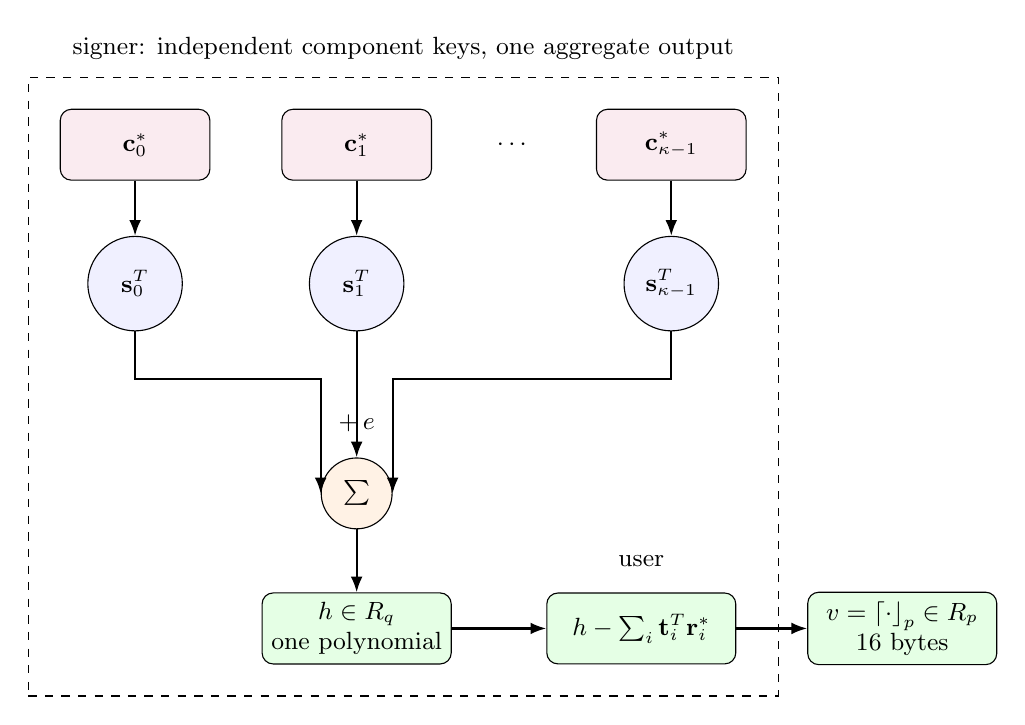
\begin{tikzpicture}[
  font=\small,
  node distance=7mm and 9mm,
  input/.style={draw,rounded corners,align=center,fill=purple!8,
                minimum width=19mm,minimum height=9mm},
  mult/.style={draw,circle,align=center,fill=blue!6,minimum size=12mm},
  op/.style={draw,circle,fill=orange!10,minimum size=9mm},
  result/.style={draw,rounded corners,align=center,fill=green!10,
                 minimum width=24mm,minimum height=9mm},
  arrow/.style={-{Latex[length=2mm]},thick}
]
\node[input] (c0) {$\mathbf c_0^*$};
\node[input,right=of c0] (c1) {$\mathbf c_1^*$};
\node[right=7mm of c1] (dots) {$\cdots$};
\node[input,right=7mm of dots] (ck) {$\mathbf c_{\kappa-1}^*$};

\node[mult,below=of c0] (m0) {$\mathbf s_0^T$};
\node[mult,below=of c1] (m1) {$\mathbf s_1^T$};
\node[mult,below=of ck] (mk) {$\mathbf s_{\kappa-1}^T$};
\draw[arrow] (c0) -- (m0);
\draw[arrow] (c1) -- (m1);
\draw[arrow] (ck) -- (mk);

\node[op,below=16mm of m1] (sum) {$\sum$};
\draw[arrow] (m0.south) -- ++(0,-6mm) -| (sum.west);
\draw[arrow] (m1.south) -- (sum.north);
\draw[arrow] (mk.south) -- ++(0,-6mm) -| (sum.east);
\node[above=2mm of sum] {$+\,e$};
\node[result,below=8mm of sum] (h) {$h\in R_q$\\one polynomial};
\draw[arrow] (sum) -- (h);

\node[result,right=12mm of h] (unblind)
 {$h-\sum_i\mathbf t_i^T\mathbf r_i^*$};
\node[result,right=of unblind] (v)
 {$v=\roundp{\cdot}\in R_p$\\16 bytes};
\draw[arrow] (h) -- (unblind);
\draw[arrow] (unblind) -- (v);

\node[draw,dashed,fit=(c0)(c1)(ck)(m0)(m1)(mk)(sum)(h),inner sep=4mm] (signerbox) {};
\node[font=\small,above=1mm of signerbox.north]
 {signer: independent component keys, one aggregate output};
\node[font=\small,above=2mm of unblind] {user};
\end{tikzpicture}%
}
\caption{One response from many lanes.  The signer evaluates each selected
commitment under its lane key and returns only their sum, with a small error.
The user removes the blinding terms and rounds the result to obtain $v$.}
\label{fig:aggregate-flow}
\end{figure}

\subsection{Finishing and presenting the credential}

After checking the response proof, the user removes its blinding terms and
rounds the result:
\[
 v=\roundp{h-\sum_i\mathbf t_i^T\mathbf r_i^*}
\]
and stores
\[
 \sigma=((m_i^*,\rho_i^*)_{i=0}^{\kappa-1},v),
 \quad (m_i^*,\rho_i^*)=(m_{i,b_i^*},\rho_{i,b_i^*}).
\]
At presentation, the verifier uses its secret keys to recompute the
expected value.  It accepts exactly when
\[
 v=\roundp{\sum_i\mathbf s_i^T
        H_R(\mathsf{credential\mbox{-}lane},i,m_i^*,\rho_i^*)}.
\]
The lane hash used at presentation must not contain the issuance session
identifier.  Revealing that identifier would immediately link the credential
to its issuance.  Instead, the session identifier is bound into the branch
formation and challenge, and both issuance and presentation use the same
credential hash shown above.  An application can derive one payload from the
ordered message/tag list:
\[
 M=H_{\mathrm{final}}(\mathsf{issuer},\mathsf{type},
              (m_i^*,\rho_i^*)_{i=0}^{\kappa-1}).
\]

\section{Why honest credentials verify}

The unblinding step cancels most of the noise introduced during issuance.
For an honestly generated selected branch,
\[
 \mathbf c_i^*=B_i\mathbf r_i^*+\mathbf e_{2,i}^*+\mathbf u_i^*.
\]
Consequently,
\begin{align*}
 h-\sum_i\mathbf t_i^T\mathbf r_i^*
 &=\sum_i\mathbf s_i^T\mathbf u_i^*
   +\sum_i\left(
       \mathbf s_i^T\mathbf e_{2,i}^*
       -\mathbf e_{1,i}^T\mathbf r_i^*\right)+e.
\end{align*}
The first term is exactly what the verifier computes.  The remaining terms
are small errors.  Both sides round to the same value unless an error moves
a coefficient across a rounding boundary.

Adding lanes also adds their errors.  With independent centered errors, the
typical noise scale grows as $O(\sqrt\kappa)$; a worst-case bound can grow
as $O(\kappa)$.  We therefore cannot reuse the BLNS23 parameters without
checking the new noise bound.  We may need a larger $q$, a smaller rounding
modulus $p$, or smaller errors in each lane.

\section{What cut-and-choose guarantees}\label{sec:cut-and-choose}

Call a branch \emph{openable} if a seed regenerates it and passes every
formation check.  For a fixed table containing one openable and one malformed
branch in each of $k$ attacked lanes, a uniformly sampled challenge opens all
$k$ openable branches with probability $2^{-k}$.  Thus an attempt that passes
those checks while selecting all $k$ malformed branches has probability
\[
 \Pr[\text{accept and select all attacked branches malformed}]=2^{-k}.
\]
In particular, a table has at most one challenge that accepts while selecting
malformed branches in every lane.  Across $q_{\mathrm{chal}}$ classical
Fiat--Shamir trials, this event has probability at most
$q_{\mathrm{chal}}2^{-\kappa}$, up to binding failures and challenge bias.
This bound concerns that event alone; the splicing attack in
Section~\ref{sec:rectangle} uses only about half the lanes in each malicious
issuance.

Two successful openings of the same table under different challenges also
reveal something useful: at least one branch that stayed hidden in the first
exchange is opened in the second.  The next lemma makes this precise.

\begin{lemma}[Two-fork selected-lane extraction]
Assuming binding of the global branch commitment, two accepting transcripts
with the same branch table and distinct binary challenge vectors reveal an
opening for at least one branch selected in the first transcript, and
symmetrically for the second.
\end{lemma}

\begin{proof}
Choose an index $j$ where the challenges differ.  If the first challenge opens
$\chi_j$, it selects $1-\chi_j$.  The second challenge opens
$\chi'_j=1-\chi_j$, revealing the selected branch's seed and hence its witness.
\end{proof}

This lemma starts with two accepting \emph{transcripts}, meaning records of
what was sent in the exchanges.  It does not show how to obtain both records
while answering an attacker that chooses later requests based on earlier
answers.  It also gives no guarantee that the same lane is revealed in every
issuance.  A quantum extraction proof would need further work.  The
interactive variant uses seed tags instead, allowing a classical proof to
recover witnesses from hash queries.

All branches, lane positions, session data, and the public key must be bound
before the challenge.  Independent lane keys prevent a direct cancellation
based on sharing one secret across lanes.  The signer checks all openings
before producing any secret-dependent output and releases only the aggregate;
individual lane responses would expose a lane to a single cut-and-choose
check.  These requirements are part of the construction, not substitutes for
the aggregate security argument.

\section{Splicing attacks and lane freshness}\label{sec:rectangle}

\subsection{Reusable lane inputs}

Each lane contributes a value that depends only on its own input.  The rounded
sum, together with the tags, forms the message authentication code (MAC).
If valid inputs can be reused across issuances, an attacker
can combine three responses to make a fourth credential.  This breaks
\emph{one-more unforgeability}: after $Q$ issuances, a user should not be
able to produce credentials for $Q+1$ distinct messages.  To see the attack,
first ignore the small rounding error and define
\[
 F_i(x)=\mathbf s_i^T H_R(x),\qquad
 Y(x_0,\ldots,x_{\kappa-1})=\sum_i F_i(x_i).
\]
Here $x_i=(m_i,\rho_i)$ and $Y$ is the user's value before rounding, with
noise omitted for now.  Keep all lanes fixed except two, called $a$ and $b$.
Choose two valid inputs for each: $x_a^0,x_a^1$ and $x_b^0,x_b^1$.  These
choices form four combinations, the corners of a rectangle.  Write $Y_{uv}$
for the response using choice $u$ in lane $a$ and choice $v$ in lane $b$.
Three honest issuances give
\begin{align*}
 Y_{00}&=F_a(x_a^0)+F_b(x_b^0)+K,\\
 Y_{10}&=F_a(x_a^1)+F_b(x_b^0)+K,\\
 Y_{01}&=F_a(x_a^0)+F_b(x_b^1)+K,
\end{align*}
where $K$ is the fixed contribution of every other lane.  The user computes
\begin{align*}
 Y^*&=Y_{10}+Y_{01}-Y_{00}\\
 &=F_a(x_a^1)+F_b(x_b^1)+K=Y_{11}.
\end{align*}
Thus three issued vector credentials yield the fourth corner, which was never
issued.  All four message vectors are pairwise distinct.

In the real protocol, the user has unblinded values
\[
 \widetilde Y_{uv}=h_{uv}-\sum_i\mathbf t_i^T\mathbf r_{i,uv}
                  =Y_{uv}+\eta_{uv},
\]
where each $\eta_{uv}$ is a small correctness error.  It computes
\[
 \widetilde Y^*=\widetilde Y_{10}+\widetilde Y_{01}-\widetilde Y_{00}
 =Y_{11}+(\eta_{10}+\eta_{01}-\eta_{00})
\]
and rounds $\widetilde Y^*$.  The combined error grows by only a constant
factor.  With the correctness margin required by the scheme, it crosses a
rounding boundary only with negligible probability.  The resulting MAC for
the unqueried vector $(x_a^1,x_b^1)$ therefore verifies.

\begin{theorem}[Three-query forgery under reusable lane inputs]
For $\kappa\geq2$, suppose valid values $x_i=(m_i,\rho_i)$ may be repeated in
different issuance sessions and the correctness error remains negligible under
a three-term signed sum.  Then the coordinate-wise aggregate construction is
not one-more unforgeable: three honest issuance queries produce four
pairwise-distinct valid vector-message credentials.
\end{theorem}

\subsection{Session freshness and balanced splicing}

In the current construction, however,
\[
 \rho_{i,b}=H_\rho(\mathsf{sid},i,b,\mathbf r_{i,b},\mathbf e_{2,i,b})
\]
contains a signer-backed, globally unique $\mathsf{sid}$.  Reusing the same
$x_i=(m_i,\rho_i)$ in a second session would require finding a cross-session
preimage or collision for $H_\rho$.  The rectangle attack therefore motivates
a mandatory rule: session identifiers must never repeat within a key epoch,
and valid lane inputs must be fresh across issuance queries.  This rule
excludes the fully honest rectangle but does not establish security.  Its
enforcement must cover concurrency, rollback, and distributed replay-state
failures that could violate uniqueness.

Unique sessions still leave a way to use the same identity.  An attacker
can put an old hash vector into a malformed branch and try to keep that
branch unopened.  It need not provide a valid seed for the old input.
Divide the lanes into two disjoint sets, $A$ and $B$.  First obtain one
honest baseline response:
\[
 Y_{00}=\sum_{i\in A}F_i(x_i^0)+\sum_{i\in B}F_i(x_i^0).
\]
In a second issuance use fresh honest inputs $x_i^1$ in $A$ and copied,
malformed baseline coefficients in $B$; in a third do the converse.  Conditional
on the required Fiat--Shamir challenges, the resulting values are
\begin{align*}
 Y_{10}&=\sum_{i\in A}F_i(x_i^1)+\sum_{i\in B}F_i(x_i^0),\\
 Y_{01}&=\sum_{i\in A}F_i(x_i^0)+\sum_{i\in B}F_i(x_i^1).
\end{align*}
Again, $Y_{10}+Y_{01}-Y_{00}=Y_{11}$, even though every valid input belongs
to a fresh session.  The attacker needs the second issuance to select the
$|B|$ malformed branches and the third to select the $|A|$ malformed ones.
Splitting the lanes as evenly as possible balances these two searches.
The work is then about $2^{\kappa/2}$ classical random-oracle trials or
$2^{\kappa/4}$ generic quantum trials.  A security estimate based only on
hiding malformed branches in all $\kappa$ lanes at once would therefore
miss this cheaper attack.

\subsection{A lower bound for copying and combining responses}

Among attacks that only copy lane values and combine responses by linear
operations, the balanced attack has the best possible exponent.  To state
this claim precisely, treat each distinct lane coefficient as a separate
symbol, called an \emph{atom}.  A later use of the same atom in the same
lane is a \emph{copy}.  We consider identities that work for every possible
assignment of values to these symbols.

\begin{theorem}[Half-copy lower bound for formal linear splicing]
Let $Q\geq2$ issued aggregates be combined with nonzero coefficients
$\alpha_1,\ldots,\alpha_Q\in R_q$ to produce an unissued aggregate containing
one target atom in every lane.  If the identity holds for every assignment of
the lane atoms, then some issuance after the first contains copies in at least
$\kappa/2$ lanes.
\end{theorem}

\begin{proof}
Fix a lane and group the $Q$ occurrences according to equal atoms.  The group
containing the target atom must have coefficient sum one; every other group
must have coefficient sum zero.  Because every $\alpha_j$ is nonzero, a
zero-sum group has at least two occurrences.  At most one group---the target
group---can be a singleton.  Consequently at most
$1+\lfloor(Q-1)/2\rfloor$ different atoms occur in this lane, so at least
$\lceil(Q-1)/2\rceil$ occurrences are copies.  Summing over all $\kappa$ lanes
gives at least $\kappa\lceil(Q-1)/2\rceil$ copy incidences.  No occurrence in
the first issuance is a copy.  Averaging over the remaining $Q-1$ issuances
therefore puts at least
\[
 \frac{\kappa\lceil(Q-1)/2\rceil}{Q-1}\geq\frac\kappa2
\]
copies in one issuance.
\end{proof}

Because valid inputs are bound to their sessions, a copied atom must be in
an unopened malformed branch unless a hash collision occurs.  The theorem
therefore forces at least $\kappa/2$ challenge bits in one issuance.  Its
scope is limited to these formal identities: it does not rule out attacks
that exploit special algebraic relations between different hash vectors.

\section{What the security proof needs}\label{sec:security-targets}

A \emph{reduction} shows how an attacker against the proposed scheme could
be used to solve an existing hard problem.  It runs the attacker and
simulates the protocol, using an instance of that hard problem in place of
some secret information.

Here the underlying problem is hashed module learning with errors (HMLWE).
Its real oracle returns a secret inner product at a hashed input, plus a
small error.  Its ideal oracle returns a random value, consistently on
repeated inputs.  HMLWE says that an efficient attacker cannot tell these
oracles apart.  This property is called \emph{pseudorandomness}.

We first study a simpler game that keeps only the sum of the lane
contributions.  Let $H_i:\{0,1\}^*\rightarrow R_q^n$ be the independent
random oracles used for the lane hashes, let $\mathbf s_i\sample D_s^n$ be
the lane secrets, and let $D_E$ sample the aggregate error.  In request $j$,
the attacker chooses the coefficients $(\mathbf a_{j,i})_i$.  The set $V_j$
contains the lanes where the reduction knows a hash input $x_{j,i}$ such that
\[
 \mathbf a_{j,i}=H_i(x_{j,i})\qquad(i\in V_j).
\]
Each such pair $(i,x_{j,i})$ must be new among accepted issuance requests.
The attacker can choose the other coefficients freely, using anything it
learned from earlier answers.  The real aggregate response is
\[
 z_j=\sum_i\mathbf s_i^T\mathbf a_{j,i}+e_j,
 \qquad e_j\sample D_E;
\]
the ideal response is chosen uniformly at random from $R_q$, independently
of earlier responses.  The attacker's goal is to tell which kind of answers
it receives.  Its \emph{distinguishing advantage} measures how much its
output probabilities differ between the two games.

Connecting this game to the full protocol requires more work.  The reduction
must also simulate the public keys, blinding terms, and response proofs, and
justify the error distribution $D_E$.  Cryptographic proofs often make these
changes through a sequence of intermediate games, called \emph{hybrids}.

\subsection{Why one fixed valid lane is enough}\label{sec:fixed-lane}

The reduction knows all lane keys except one.  For that lane, it asks its
HMLWE oracle for the required contribution and adds the other contributions
it can compute itself.  This works whenever the selected input in that lane
is hash-derived and its hash input is known.

\begin{lemma}[Fixed valid lane]
Suppose a fixed index $i^*$ belongs to $V_j$ in every aggregate query.  Then
the restricted aggregate game reduces to ordinary HMLWE for lane $i^*$.
\end{lemma}

\begin{proof}
Use the unknown HMLWE secret as the key for lane $i^*$, and generate the
other lane keys locally.  On request $j$, the label $x_{j,i^*}$ has not been
used in an earlier accepted request.  Obtain
$b_j=\mathbf s_{i^*}^T H_{i^*}(x_{j,i^*})+e_j$ from the HMLWE oracle and return
\[
 b_j+\sum_{i\ne i^*}\mathbf s_i^T\mathbf a_{j,i}.
\]
With a real HMLWE oracle, this is exactly the real aggregate response.  With
an ideal oracle, $b_j$ is a fresh uniform value.  Adding the other
contributions leaves the result uniform.  Even malformed inputs in the
other lanes can be handled because the reduction knows those lane keys.
\end{proof}

\begin{corollary}[All lanes valid]
If $V_j=[\kappa]$ in every query, the aggregate game reduces to ordinary
HMLWE, and hence to MLWE in the random-oracle model by BLNS23 Lemma~4.3.
\end{corollary}

\begin{proof}
Choose any fixed lane and apply the lemma.
\end{proof}

The same lane must work throughout the entire issuance history.  For example,
if the reduction uses lane 2, it needs lane 2 to stay valid in every accepted
request.  A request that is valid only in lane 3 does not help it: it knows
lane 3's key already, but still cannot compute an arbitrary input under lane
2's unknown key.  The HMLWE oracle accepts hash inputs, not arbitrary
coefficient vectors.  Section~\ref{sec:interactive} explains how the
four-message variant keeps one fixed lane usable across all issuances.

\subsection{The two security goals for the two-message proposal}

The first goal is to show that the aggregate responses look random.  The
game must follow the real protocol's order: the attacker commits first, and
only then learns the challenge.  In request $j$, it fixes a unique session
identifier and all branch coefficients
\[
 (\mathbf a_{j,i,0},\mathbf a_{j,i,1})\qquad(i\in[\kappa])
\]
under one binding global digest $C_j$.  The challenge is then
$\boldsymbol\chi_j=H_{\mathrm{chal}}(\mathsf{sid}_j,C_j)$.
The attacker opens branch $\chi_{j,i}$ in every lane.  The verifier checks
that each opened branch was formed correctly for this session.  If all
openings pass, the real game returns
\[
 z_j=\sum_i\mathbf s_i^T\mathbf a_{j,i,1-\chi_{j,i}}+e_j,
\]
while the ideal game returns a fresh uniform ring element.  Hash-derived
selected inputs must use fresh labels in their lanes.  All challenge-hash
queries count toward $q_{\mathrm{chal}}$, including attempts the attacker
discards.  We call this goal \emph{transcript-causal aggregate HMLWE}
(tc-AHMLWE); ``transcript-causal'' means that the game respects the order of
the exchange.  This goal remains unproved for the two-message proposal.

The second goal is to prevent extra credentials.  Random-looking issuance
responses alone are not enough, because the function
\[
 F(\mathbf x)=\sum_i\mathbf s_i^T H_i(x_i)
\]
still has the rectangle relation from Section~\ref{sec:rectangle}.  The
security game must also model the verifier's actual interface: it accepts or
rejects a proposed credential without revealing the correct value of $F$.

We call this second game \emph{transcript-causal one-more hidden linear
functions} (tc-OMHLF).  It lets the attacker make issuance requests in the
order above and test proposed credentials with
\[
 \mathsf{Check}(\mathbf x,v)=
 \left[v=\roundp{\sum_i\mathbf s_i^T H_i(x_i)}\right].
\]
After at most $Q$ accepted issuances, the attacker wins by producing $Q+1$
distinct vectors $\mathbf x^{(r)}$, each with a value $v^{(r)}$ that passes
$\mathsf{Check}$.  Individual lane inputs may repeat between these vectors.
Allowing this reuse is necessary to cover splicing attacks.

We could assume directly that winning this game is infeasible, but that would
be a new assumption specific to this protocol.  We do not have a reduction
from ordinary HMLWE for the two-message game.  Formally, the desired winning
probability is \emph{negligible}: as $\lambda$ grows, it eventually becomes
smaller than $\lambda^{-c}$ for every fixed positive constant $c$.

\section{A four-message variant}
\label{sec:interactive}

Here the signer chooses the challenge after the user commits.  We combine
the parallel-instance argument of Chairattana-Apirom et al.~\cite{PCC22}
with the fixed-lane lemma from Section~\ref{sec:fixed-lane}.  The aim is to
keep one lane valid for every accepted request.  That proves a result for
the simplified response game.  To extend the argument to extra credentials,
we then bind all lanes to one hidden message.

\subsection{Recovering seeds and limiting cheating attempts}

First, attach a hash of the seed to every branch:
\[
 d_{r,i,b}=H_{\mathrm{seed}}(\mathsf{sid}_r,i,b,z_{r,i,b}),
\]
and bind every tag $d_{r,i,b}$ together with its branch vector
$\mathbf c_{r,i,b}$ under the global digest.  The user sends the selected tag and vector,
and opens every other branch by revealing its seed.

In the classical ROM, the reduction can observe the attacker's hash queries.
It searches that history for the selected tag, recovers the seed, and
reconstructs the branch.  This is why we call the tag \emph{extractable}.
The real signer has no such access to the user's hash queries, so the selected
seed stays private.  A branch is \emph{known-valid} if the seed appeared in
a hash query before the digest was fixed and expanding it passes every
formation check.

Use $g$ lanes, also called \emph{components}, with independent keys.  Let
$q_{\max}$ be the maximum number of interactions started within one key
epoch.  A counter $r$ advances whenever an interaction starts, including
ones that later abort.  Counter updates must be atomic so that concurrent
requests cannot reuse a value.

In interaction $r$, prepare $A_r$ branches per lane and commit to all of
them.  The number of branches per lane is called the \emph{arity}.  Only
after receiving the commitment does the signer choose an independent uniform
selected index $J_{r,i}\in[A_r]$ for each lane.  All other branches are
opened.  We choose the arity schedule so that the sum of the per-attempt
cheating probabilities stays small:
\[
 \sum_{r=1}^{q_{\max}}\frac1{A_r}\leq\frac1{3\vartheta};
 \qquad
 A_r=\left\lceil
   3\vartheta\ln(q_{\max}+1)(r+1)
 \right\rceil
\]
The displayed choice of $A_r$ satisfies this bound.  The parameter
$\vartheta>1/3$ controls how small the bound is.  Increasing the arity over
time makes each later attempt less likely to hide a malformed branch.
A sufficiently large fixed arity would also work if $q_{\max}$ is known.

Call an accepted request a \emph{cheat in component $i$} if its selected
branch in that lane is not known-valid.  An \emph{untouched} component is
one where no such cheat occurs during the whole history.  The next lemma
bounds the chance that the attacker cheats in every lane at least once.
Aborting after seeing a challenge still consumes the counter value.

\begin{lemma}[Untouched component]
Let $\vartheta>1/3$.  In the
unpredictable-challenge experiment above, the probability that every one of
the $g$ components is cheated in at least once is at most
\[
 (3\vartheta)^{-g}+\varepsilon_{\mathrm{ext}},
\]
where $\varepsilon_{\mathrm{ext}}$ covers random-oracle preimage and global
binding failures.
\end{lemma}

\begin{proof}
Consider the fixed branch table just before the signer chooses its indices.
Except for extraction or binding failures, a request can pass only if each
lane has at most one branch that is not known-valid: all other branches must
be opened and checked.  A successful cheat must leave that one branch hidden,
which happens with probability at most $1/A_r$.

To bound the total risk in one lane, compare these attempts with independent
trials that succeed with probability $1/A_r$ in interaction $r$.  These
trials can only overestimate the chance of a successful cheat.  The chance
that at least one succeeds is
\[
 1-\prod_r(1-1/A_r)\leq\sum_r1/A_r\leq1/(3\vartheta).
\]
This comparison still works when the attacker adapts to earlier answers.
Before each challenge, mark the branch whose selection could produce an
accepted cheat.  If there is no such branch, mark any fixed branch for the
comparison alone.  Selecting the marked branch counts as a success in the
comparison even when the real request would be rejected.

Each fresh index hits its marked branch with probability $1/A_r$, whatever
the earlier history.  The indices in different lanes are sampled
independently.  Thus the comparison trials are independent across lanes and
interactions, and their chance of hitting every lane at least once is at
most $(3\vartheta)^{-g}$.  Extraction and binding failures contribute the
additional term $\varepsilon_{\mathrm{ext}}$.
\end{proof}

\subsection{Why the aggregate can look random}

Call the response-only game for this variant \emph{uc-AHMLWE}, where ``uc''
stands for unpredictable challenge.  It uses the $g$ lanes, seed tags, arity
schedule, and signer-chosen indices just described.  Valid selected labels
must be new among accepted issuances.  In the ideal game, each accepted
aggregate response is replaced by an independent uniform ring element.

The untouched-component lemma lets us use the fixed-lane reduction.  The
bound below adds the loss from choosing a lane to the chance that no lane
stays untouched.  The notation $\operatorname{Adv}$ denotes distinguishing
advantage.

\begin{theorem}[Unpredictable-challenge aggregate HMLWE]
For every classical distinguisher $\mathcal A$ against uc-AHMLWE, there is an
ordinary HMLWE distinguisher $\mathcal B$ such that
\[
 \operatorname{Adv}_{\mathrm{uc\text{-}AHMLWE}}(\mathcal A)
 \leq
 g\,\operatorname{Adv}_{\mathrm{HMLWE}}(\mathcal B)
 +2(3\vartheta)^{-g}+2\varepsilon_{\mathrm{ext}}.
\]
Consequently, in the ROM the restricted aggregate problem reduces to MLWE by
BLNS23 Lemma~4.3.
\end{theorem}

\begin{proof}
Unless the preceding lemma's bad event occurs, at least one lane is
untouched.  In that lane, every selected branch of an accepted request is
known-valid.  Group these histories by the lowest-index untouched lane.
For one such group, place the HMLWE challenge in that lane and generate all
other keys locally.  If that lane is ever cheated in, abort the simulation.
Otherwise, its extracted seed gives a fresh input for the HMLWE oracle.

Add the other lanes' contributions as in the fixed-lane lemma.  A real
oracle produces the real aggregate response; an ideal oracle makes the sum
uniform.  Splitting histories into at most $g$ groups costs a factor of at
most $g$.  Excluding the bad event from both games costs at most twice its
probability, giving the stated bound.
\end{proof}

\subsection{Binding all lanes to one message}\label{sec:common-message}

A new message vector need not contain a new input in our fixed lane.  The
rectangle attack illustrates the problem: it forms a new combination using
only inputs that have already appeared.  To rule out extra credentials by
the fixed-lane argument, we need a new output message to require a new hash
input in that lane.

We obtain this property by making all lanes refer to the same hidden message
$M$.  Use a commitment $\mathsf{Com}$ with three properties: it hides $M$;
it cannot be opened to two different messages (\emph{binding}); and anyone
can rerandomize it without knowing $M$, while preserving the committed
message.  Write $\phi_0$ for its initial randomness and set
\[
 \mu_0=\mathsf{Com}(M;\phi_0),\qquad
 \mu_{i,b}=\mathsf{Translate}(\mu_0;\Delta_{i,b})
           =\mathsf{Com}(M;\phi_0+\Delta_{i,b}),
\]
where the branch seed determines $\Delta_{i,b}$, the change to the commitment's
randomness.  The seed also determines the lattice witnesses.  Branches now contain
commitments to the same message, instead of separately generated messages.
The global digest includes $\mu_0$, and the lane hash becomes
$H_i(\mu_{i,b},\rho_{i,b})$.

When a branch is opened, the signer checks that its commitment is the
required rerandomization of $\mu_0$.  It can do this without learning $M$.
At presentation, the user reveals $M$, the selected commitment randomness
$\phi_i=\phi_0+\Delta_{i,J_i}$, the tags $\rho_i$, and the rounded aggregate
value.  The verifier reconstructs each $\mu_i=\mathsf{Com}(M;\phi_i)$ and
checks the aggregate using $H_i(\mu_i,\rho_i)$.  The selected branch seeds
stay private.

Binding means the same commitment cannot open to two different messages.
So credentials for distinct messages must have distinct $\mu_i$ in every
lane, including the untouched one.  After $Q$ accepted issuances, at most
$Q$ HMLWE inputs in that lane have received issuance evaluations.  Producing
credentials for $Q+1$ distinct messages must require at least one new
evaluation.  The attacker may already know the public hash at that input;
what it lacks is the secret-key evaluation.

In the final ideal game, that missing evaluation is random.  The BLNS23
argument bounds the chance of guessing its rounded value by $q_V2^{-h}$,
where $q_V$ is the number of verification attempts.  Here $h$ is an entropy
bound, not the response polynomial: no rounded value has probability greater
than $2^{-h}$.  Assuming commitment binding, correctness, and the remaining
BLNS23 simulation steps, this gives
\[
 \operatorname{Adv}_{\mathrm{OM}}(\mathcal A)
 \leq
 g\,\operatorname{Adv}_{\mathrm{HMLWE}}(\mathcal B)
 +2(3\vartheta)^{-g}+2\varepsilon_{\mathrm{ext}}
 +\operatorname{Adv}_{\mathrm{bind}}+q_V2^{-h}
 +\varepsilon_{\mathrm{hyb}}+\varepsilon_{\mathrm{corr}}.
\]
The terms $\operatorname{Adv}_{\mathrm{bind}}$,
$\varepsilon_{\mathrm{hyb}}$, and $\varepsilon_{\mathrm{corr}}$ account for
breaking commitment binding, distinguishing the intermediate simulations,
and correctness failures.  These parts still need to be established for a
concrete protocol.  The common-message commitment supplies the counting step:
an extra distinct message forces a new input in the fixed lane.

\subsection{What this result covers and what it costs}

Issuance now takes four messages: commit to the table, receive the signer's
challenge, send the openings, and receive the response and proof.  Every
started interaction consumes a counter value, including abandoned attempts.
The extraction argument observes classical hash queries; extending it to
quantum queries requires a separate theorem.

The signer must choose the challenge after the user commits.  If we replace
this step with Fiat--Shamir, the user can try $L$ candidate digests locally.
Its chance of selecting a malformed branch in one lane rises from $1/A_r$
to $1-(1-1/A_r)^L$.  The user can repeat this search for each lane, and the
signer never sees the discarded attempts.  When the arity is polynomial,
polynomially many trials suffice to target every lane this way.

This is not itself a forgery.  It does, however, remove the guarantee that
one lane stays untouched.  The four-message proof therefore does not transfer
to the Fiat--Shamir proposal.

To complete the one-more proof, we still need a concrete commitment scheme,
the public-key and response-proof simulations, and the correctness bound.
We must also prove blindness separately.  The extra tags, commitments,
openings, and changing branch counts have costs that are not included in the
two-message proposal's size estimates.

\section{Why privacy may hold, and what remains to prove}

In the two-message proposal, the issuer sees the opened decoy branches during
issuance.  The credential contains the other messages.  When the credential
is presented, the issuer learns $(m_i^*,\rho_i^*)_i$.  It can subtract their
hashes from a stored issuance request and test whether that request might
have produced the credential.  This leads to the question of whether
\[
 \mathbf c_i^*-H_R(m_i^*,\rho_i^*)
   =B_i\mathbf r_i^*+\mathbf e_{2,i}^*
\]
holds for some short, unknown blinding vectors.  The intended MLWE argument
is that recognizing this relation is hard.  If opened and selected messages
also have indistinguishable distributions, this suggests that the issuer
cannot tell which issuance produced a presented credential.  A complete
blindness proof must make that argument precise.

A dishonest issuer may try to mark credentials by using malformed keys or
specially chosen errors.  The response proof must link every lane key to the
public parameters and bound the aggregate error.  One option is to prove
that the error came from the required secret pseudorandom function, but this
adds a nonlinear computation to the proof.  Another is to show that every
allowed error disappears under rounding except with negligible probability.
The analysis must also rule out \emph{selective failure}: causing particular
requests to fail so that later behavior reveals which credential was issued.

For the common-message variant, privacy must still hold after the user
reveals the selected commitment openings at presentation.  The aggregate
hardness theorem alone does not show that these openings leave the issuance
session hidden.

\section{What remains to be proved}\label{sec:open}

\begin{enumerate}
 \item \textbf{Security of the two-message proposal.} Prove both goals from
Section~\ref{sec:security-targets}: responses should look random, and a user
should not obtain extra credentials.  Account for adaptive requests,
classical and quantum hash queries, grinding, multiple targets, and splicing.
 \item \textbf{Connecting the interactive game to the full protocol.}
Complete the simulations of public keys, blinding terms, response proofs,
and verification answers.  Choose a commitment scheme with the hiding,
binding, and rerandomization properties used in the one-more argument,
including suitable bounds on its randomness and openings.
 \item \textbf{Sessions and counters.} Keep session identifiers unique.
For the interactive variant, enforce the attempt counter and branch-count
schedule even under simultaneous requests, deliberate aborts, crashes,
rollback, and multiple signer replicas.
 \item \textbf{Privacy against a dishonest issuer.} Rule out linking through
keys, errors, failed requests, or later presentation.  Supply a sound
zero-knowledge response proof, and justify how public matrices are generated
and keys are checked.
 \item \textbf{Choosing secure parameters.} Analyze lattice hardness, the
sum of lane errors, and rounding failures together.  The starting value
$\kappa=512$ only addresses the generic balanced quantum splice.  A full
128-bit bound and realistic efficiency estimates are still needed for each
variant and branch count.
 \item \textbf{Returning only the intended output.} Check all openings before
returning any secret-dependent value.  Ensure that partial sums, individual
lane responses, failure details, and timing reveal no extra information.
\end{enumerate}

\section{Estimated communication and computation costs}\label{sec:efficiency}

These estimates cover the two-message proposal, including an optional version
with more branches per lane.  They do not include the four-message variant's
seed tags, common-message commitments, or changing branch counts.

The user prepares $2\kappa$ lattice branches, commits to them with one
digest, and opens $\kappa$ by sending their seeds.  With $\kappa=256$, this
means 512 branches and 256 openings.  The quantum starting point
$\kappa=512$ doubles both counts.  The signer checks the opened branches and
computes one aggregate response.  Its proof covers more relations than the
single-lane BLNS23 response proof, but those relations can be handled together
and contain only lattice arithmetic and size bounds.

\subsection{Bytes sent and stored}

For this size calculation, use the BLNS23 keyed-verification values
$d=64$, $n=93$, $\lceil\log_2q\rceil=152$, $p=4$, and 32-byte messages and
tags.  We take $\kappa=512$ as the minimum starting point for 128-bit
post-quantum resistance to the balanced Fiat--Shamir splice.  Ring elements are packed at
152 bits per coefficient.  Branch openings are 32-byte seeds and the single
global branch commitment is a 48-byte digest.

One commitment vector has exact packed length
\[
 |\mathbf c|=nd\lceil\log_2q\rceil
 =93\cdot64\cdot152=904{,}704\text{ bits}=113{,}088\text{ bytes}.
\]
Only the $\kappa=512$ unopened vectors are transmitted in full, occupying
57,901,056 bytes.  The global commitment occupies 48 bytes and the 512 opened
seeds occupy 16,384 bytes.  With a 32-byte session identifier, the exact fixed
portion of the first message is therefore 57,917,520 bytes (55.23 MiB).
The challenge is recomputed and is not transmitted separately.  Relative to
transmitting all commitment vectors and explicit witnesses, seeded openings
reduce the first message by approximately 52.5\%.

The aggregate response $h\in R_q$ occupies
\[
 |h|=d\lceil\log_2q\rceil=64\cdot152=9{,}728\text{ bits}
 =1{,}216\text{ bytes}.
\]
The second message has length $1{,}216+|\pi_{\mathrm{resp}}|$ bytes.  To give an exact
total, we need an actual zero-knowledge proof for all the response relations.
A suitable construction could use LaBRADOR~\cite{BS22}, but the equations
alone do not determine the proof size.

\begin{table}[htbp]
\centering
\begin{tabular}{lr}
\toprule
Wire component & Bytes \\
\midrule
512 unopened commitment vectors & 57,901,056 \\
One 48-byte global commitment & 48 \\
512 32-byte opened seeds & 16,384 \\
Session identifier & 32 \\
User $\rightarrow$ signer, fixed total & 57,917,520 \\
Aggregate $h$ & 1,216 \\
Signer $\rightarrow$ user & $1,216+|\pi_{\mathrm{resp}}|$ \\
MAC $(\rho_0,\ldots,\rho_{511},v)$ & 16,400 \\
MAC plus 512 32-byte messages & 32,784 \\
\bottomrule
\end{tabular}
\caption{Preliminary exact wire sizes with seeded openings and one 384-bit
global branch commitment under the stated canonical encoding.
The batched response proof is not yet instantiated.}
\label{tab:wire-size}
\end{table}

The MAC calculation uses 512 tags of 32 bytes and
$d\log_2p=128$ bits for $v$:
\[
 |\mathsf{MAC}|=512\cdot32+16=16{,}400\text{ bytes}.
\]
If the messages are considered part of the stored credential rather than
external signed data, 16,384 additional bytes give a 32,784-byte credential.

\subsection{Optional tradeoff: more branches per lane}

Two branches per lane give the simplest protocol and security game.  Using
more branches is an optional way to reduce bandwidth, at the cost of more
computation.  Its security analysis should follow a proof of the binary
proposal.

Most of the first message consists of full lattice vectors.  We can send
fewer of these by using groups of $A=2^a$ branches.  Fiat--Shamir selects one
branch per group to stay hidden; the other $A-1$ are opened with 32-byte
seeds.  With $g$ independently keyed groups, hiding one malformed branch in
every group succeeds with probability
\[
 A^{-g}=2^{-ag}.
\]
The balanced splice constrains about half of the groups, so its generic quantum
cost is approximately $2^{ag/4}$.  For a 128-bit post-quantum target we
therefore require $ag\geq512$.  Only $g$ full lattice vectors are then
transmitted.  Ignoring
the response proof, the fixed first-message size is
\[
 g|\mathbf c|+g(A-1)\cdot32+48+32\text{ bytes},
 \qquad g=\left\lceil\frac{512}{\log_2 A}\right\rceil.
\]

\begin{table}[htbp]
\centering
\begin{tabular}{rrrrr}
\toprule
$A$ & $g$ & challenge bits & generated branches & first message \\
\midrule
2   & 512 & 512 & 1,024  & 55.23 MiB \\
4   & 256 & 512 & 1,024  & 27.63 MiB \\
16  & 128 & 512 & 2,048  & 13.86 MiB \\
32  & 103 & 515 & 3,296  & 11.21 MiB \\
64  & 86  & 516 & 5,504  & 9.44 MiB \\
256 & 64  & 512 & 16,384 & 7.40 MiB \\
512 & 57  & 513 & 29,184 & 7.04 MiB \\
1024& 52  & 520 & 53,248 & 7.23 MiB \\
\bottomrule
\end{tabular}
\caption{Bandwidth/computation tradeoff for higher-arity cut-and-choose.
The branch count approximates user generation and signer opening work.}
\label{tab:arity}
\end{table}

For bandwidth alone, the stated parameters are minimized near $A=512$, where
the first message is 7,378,160 bytes (7.04 MiB): 57 full vectors consume
6,446,016 bytes, 29,127 opened seeds consume 932,064 bytes, and the global
commitment plus session identifier consume 80 bytes.  The corresponding MAC
contains 57 tags and one 16-byte rounded value, hence
\[
 57\cdot32+16=1{,}840\text{ bytes}.
\]
This setting requires generating and checking 29,184 branches, however, versus
1,024 in the binary construction.  Values such as $A=16$ or $A=32$ may therefore
give a better end-to-end tradeoff: they reduce issuance to 13.86 or 11.21 MiB
while increasing branch computation by only two to three times.  A benchmark
must include deterministic expansion, hash-to-ring, matrix--vector products,
and response-proof scaling before selecting $A$.

The earlier two-transcript argument still works.  If two accepted openings
of the same table select different indices in a group, the second reveals
the branch hidden in the first.  The challenge now has $A$ choices per group,
and the digest must still bind every branch.

Changing the branch count also changes the keys and the equations.  The
binary proposal has $\kappa=512$ independent lane secrets:
\[
 (\mathbf s_0,\ldots,\mathbf s_{511})
     \in (R_q^n)^{512}.
\]
In the $A$-ary scheme there are only $g=\lceil512/\log_2A\rceil$ component
secrets,
\[
 (\mathbf s_0,\ldots,\mathbf s_{g-1})
     \in (R_q^n)^g,
 \qquad
 h=\sum_{i=0}^{g-1}\mathbf s_i^T\mathbf c_i^*+e.
\]
Fewer lane keys mean smaller keys, fewer terms and errors in the aggregate,
fewer response-proof relations, and fewer message/tag pairs in the MAC.
Each lane key still uses the full BLNS23 module dimension.  Only the number
of separately keyed groups changes.  We must therefore check correctness,
lattice hardness, and parameters again for each choice of $A$.

The credential still stores $\kappa$ message/tag pairs in the binary version,
or $g$ in the higher-arity version, unless a safe compression method is found.
Any comparison should include those bytes as well as the issuance traffic,
proof-generation and checking times, presentation time, key sizes, and
rounding-failure probability.

\section{Conclusion}

Cut-and-choose offers a way to avoid proving hash computations inside the
user's first message.  The user opens some branches for checking, and the
signer returns one sum under independent lane keys.  But summing separate
lane contributions also enables splicing attacks.  Unique sessions block
the fully honest rectangle attack; balanced splicing still costs about
$2^{\kappa/2}$ classically or $2^{\kappa/4}$ with generic quantum search.
These attacks set a minimum lane count for resisting them.  Security of the
two-message proposal remains open.

The four-message variant has a more direct proof route.  The signer chooses
what to check after commitment, and a counted schedule limits the total
chance of cheating in each lane.  Seed tags let the classical reduction
recover the selected witnesses.  With high probability, one fixed lane
remains valid throughout, allowing the simplified response game to reduce to
ordinary HMLWE.  Binding every lane to the same hidden message then makes an
extra distinct-message credential require a new evaluation in that lane.
The remaining work is to connect this game to the full protocol, prove
privacy, and choose concrete secure parameters.  The two-message proposal
needs its own reduction that handles the user's ability to grind challenges.

\begin{thebibliography}{9}
\bibitem{BLNS23}
W.~Beullens, V.~Lyubashevsky, N.~Nguyen, and G.~Seiler.
\newblock Lattice-Based Blind Signatures: Short, Efficient, and Round-Optimal.
\newblock IACR Cryptology ePrint Archive, Report 2023/077, 2023.
\newblock \url{https://eprint.iacr.org/2023/077}.

\bibitem{PCC22}
R.~Chairattana-Apirom, L.~Hanzlik, J.~Loss, A.~Lysyanskaya, and B.~Wagner.
\newblock $\Pi$-Cut-Choo and Friends: Compact Blind Signatures via Parallel
Instance Cut-and-Choose and More.
\newblock IACR Cryptology ePrint Archive, Report 2022/007, 2022.
\newblock \url{https://eprint.iacr.org/2022/007}.

\bibitem{BS22}
W.~Beullens and G.~Seiler.
\newblock LaBRADOR: Compact Proofs for R1CS from Module-SIS.
\newblock IACR Cryptology ePrint Archive, Report 2022/1341, 2022.
\newblock \url{https://eprint.iacr.org/2022/1341}.

\end{thebibliography}

\end{document}
